\chapter{Physics of neutron star interiors} 
\chapterimage[width=15cm]{wordcloud/chap2b.png}
In this chapter, we will study the neutron star interiors in more detail.
In practice, this means describing the behavior of the matter from a densities of $\sim 10^{-2} \gcm$ to $\sim 10^{16} \gcm$, an impressive $18$ orders of magnitude range starting from a hot and rarefied electron corona to an ultra-dense neutron liquid.

The structure of the star can be roughly divided into three distinct sections: atmosphere, crust, and core.
Neutron star atmosphere holds a negligible amount of matter in comparison to the whole star, but it is important for the radiative processes.
It is the radiation from the atmosphere that we actually observe.
%Both the crust and the core are typically divided into to two different layers that we call the outer and inner parts.
The crust, like the name implies, can be understood as a solidified layer surrounding the liquid core.
Physics describing the crust is relatively well known and same type of matter consisting of ions, protons, and electrons can be found inside white dwarf stars.
Bulk of the mass, on the other hand, is located on the liquid neutron core.
Detailed microphysics of such matter are still unknown and this is reflected in a large uncertainty in the actual size of the star that is still unconstrained.

We begin by giving an overview of the characteristics of each of the different layers.
By combining this information, we can then build different models for the neutron stars and describe some more global aspects of them such as mass and radius.
For this we need to solve the relativistic equations of hydrostatic equilibrium, that are also discussed.
In the end, this enables us to build a mapping between the (un)known microphysics of the dense matter and the astrophysical observables.


\section{Equation of state}
%Often means dependency between $P$ and $\rho$. 
%Or sometimes the associated energy density $\epsilon = \rho c^2$.
%Also depends on $T$ but composed mainly on strongly degenerate fermions so so temperature dependency is negligible.
%
%Bulk property of the sea of fermions.
%
%Eos for $\rho > \nsat$ can not be produced in laboratory.
%Can not be calculated because of the lack of precise many-body theory of strongly interacting particles.
%
%
%Baryon mass $M_b$ that is sum of baryon masses.
%Gravitational mass $M$ that is $M_b$ from where the gravitational binding energy is subtracted. \cite{Zwicky38}

In thermodynamics, we speak of \emph{state variables} that describe a current state of the matter under a given physical conditions.
These include, for example, the density $\rho$, pressure $P$, and temperature $T$ of the matter.
Equation of state is a thermodynamical equation connecting these states variables together.
Often, when focusing on neutron stars, what we mean by EoS is a function connecting the pressure and the density of the matter only, $P(\rho)$.

The dependency on the rest of the variables such as temperature can be often forgotten because the matter is \emph{degenerate}.%
\mnote{Degenerate matter}
In contrast to the ``normal'' matter where a statistical moments such as temperature can be used to describe a large ensemble of particles, the degenerate matter is dominated by quantum mechanical effects of single particles.
Because of the immense densities, a free particle in a degenerate matter is actually bounded into a finite volume.
Inside this small volume, the energy levels of the particle are restricted to take only a discrete set of values called quantum states, because of the underlying wave-nature of the quantum mechanical description.
Hence, a notion of temperature, for example, does not make much sense.

Overview of the EoS for the full range of densities relevant to neutron stars is shown in \fig{fig:eos}.
Another perspective is shown in \fig{fig:slice} that visualizes the dependency of the pressure and cumulative mass of the star against the radial coordinate as measured starting from the core.
From here it is easy to see that temperature only plays a role in the very uppermost $\sim 10\,\mathrm{meters}$ of the atmosphere.
Behavior of the matter is also quite well known all the way up to the crust-core interface, after which we start to see larger deviations because of the different EoS models.
In the Earthly laboratories we can probe the matter somewhere close to $10^{14} \gcm$, after which the densities becomes too great for us to handle in.%
\footnote{Maximum densities reached in the Earth are usually obtained by colliding heavy nucleons together, momentarily creating a core of even denser matter.
The densest naturally occurring element found on top of planet Earth is osmium that has a density of ``just'' $\rho \approx \Ten{2.2}{1}\gcm$.
}
On the other hand, it is exactly starting from this density range that the bulk of the neutron star just starts.
Another curious quirk of Nature is how all of the complicated microphysics gets reduced to simple line segments in the logarithmic scales, also known as polytropic pressure relations.
In the following sections, we will focus on deriving these simple relations as it helps us in understanding the underlying physics.


\begin{figure}
\centering
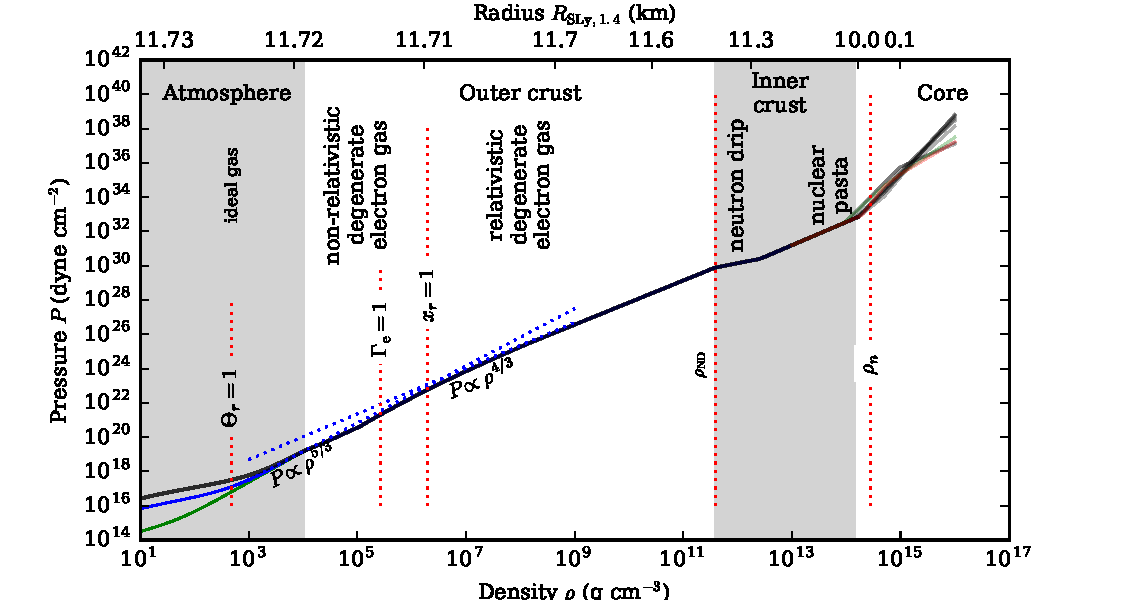
\includegraphics[width=17cm]{notes/eos/eos.pdf}
\caption{\label{fig:eos}
Overview of the pressure versus density relation for the full range of densities relevant for neutron stars.
Here the evolution of the pressure is shown against the densities depicted in the bottom vertical axis.
Green solid line shows the EoS for matter at $T=10^6\Kelvin$, whereas blue line is for $T=\Ten{5}{6}\Kelvin$, and black for $T=10^7 \Kelvin$.
Additionally, the upper vertical axis shows the evolution of the radial coordinate computed for one particular EoS (SLy, see \sect{sect:core}) and neutron star configuration (mass of $1.4\Msun$).
Different shaded vertical regions show the corresponding interior structures of the star.
Additionally, some interesting densities are highlighted with dashed red lines and text labels (see Sects.~\ref{sect:atmos}$-$\ref{sect:core}).
}
\end{figure}


\begin{figure}
\centering
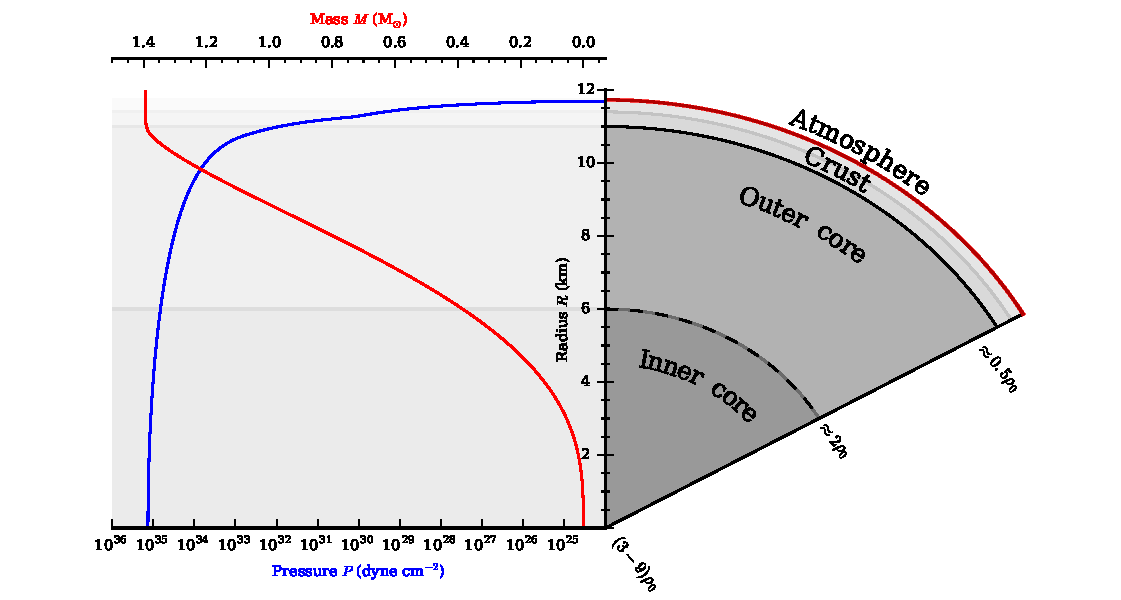
\includegraphics[width=17cm]{figs/slice/slice.pdf}
\caption{\label{fig:slice}
Overview of the neutron star structure.
Right side of the figure shows a schematic presentation of the star's interiors against the radial coordinate, whereas the left side shows the pressure (blue; bottom axis) and cumulative mass (red; top axis) evolution from the core to the surface.
}
\end{figure}


\section{Atmosphere}\label{sect:atmos}
%Thin layer of plasma
%From centimeters in hot to millimeters in cold 
%Zavlin \& Pavlov 2002\cite{ZP02}
%\cite{Potekhin14}
%Where spectrum or thermal electromagnetic radiation is formed.
%Spectrum, beaming and polarization of emerging radiation can be determined from radiation transfer problem in atmospheric layers.
%thermal bb 
%magnetosphere powerlaw-like
%radiation espaces to the surrounding space without considerable losses.
%Gaseous uppermost layers.
%For strong magnetic field strenghts and low temperatures, the hydrogen can condensate into a liquid or solid surface.
%This is, however, quite rare and usually the hydrogen remains gaseous forming an atmosphere.

Atmosphere of a star is the first and uppermost layer responsible for the emergent radiation.
It consists of a thin layer of plasma and ranges from a few millimeters to couple of centimeters in height.
In most situations the plasma is in a gaseous state, but in some more rare cases when the magnetic field is extraordinarily strong and the temperature is low, the plasma can condensate into a liquid or a solid surface.
Such condensed surfaces are, however, rare and usually the gaseous description is more than enough.\cite[for a review, see][]{ZP02, Potekhin14}

%Observationally we usually see either thermal radiation originating directly from the star's atmosphere, or a non-thermal power-law like component from the surrounding magnetosphere, or a combination of both.\cite[for a review, see][]{ZP02, Potekhin14}
%Properties of emergent radiation strongly depend on the chemical composition of the atmosphere.
%Difference to normal stars is that we only expect the composition to consist of the lightest element as heavier ones sink to the bottom.\cite{AI80}
%Consequence of gravitational force.

Properties of the emergent thermal radiation strongly depend on the chemical composition of the atmosphere.
In the atmospheres of normal stars the composition is a mixture of multiple elements.
The most stable chemical element on the surface of a neutron star is iron.
However, even a small accreted mass of $10^{-17}\Msun$, originating from the surrounding interstellar medium, is enough to cover the whole star, and hence a variety of elements are also expected in the neutron star atmospheres.
On the other hand, the enormous gravity results in an effective separation of elements leading to a strong sedimentation of the atmosphere where the lighter elements are expected to lay on top of the heavier ones.\cite{AI80}
Hence, the atmosphere is usually expected to consist of mainly hydrogen.


The effects from the gravity can be quantified by considering a so-called compactness parameter
\be
u = \frac{ R_{\mathrm{S}} }{R}
\ee
where $R$ is the radius of the neutron star and the corresponding Schwarzchild radius is defined as
\be
R_{\mathrm{S}} = \frac{2 G M}{c^2} \approx 2.95 \frac{M}{\Msun} \km,
\ee
where $G$ is the gravitational constant, $c$ is the speed of light, and $M$ is the mass of the star.
Hence, a neutrons star has a compactness parameter in the range of $u \approx 1/5$ to $1/2$ resulting in a considerable general relativistic corrections.
In comparison, the Sun has $u \approx \Ten{4.24}{-6}$.
Gravitational acceleration under general relativistic theory is
\be
g = \frac{G M}{R^2} \frac{1}{\sqrt{1-u}} = \Ten{1.38}{14} \frac{1}{\sqrt{1-u}} \left( \frac{M}{\Msun} \right) \left( \frac{10\km}{R} \right)^2 \cmss.
\ee
Hence, a surface gravitational accelerations $g$ of $\sim 10^{14}$ to $\sim 10^{15}\cmss$ are expected for neutron stars.
By considering a barometric atmosphere we can also estimate the scale height as
\be
H_{\mathrm{a}} = \frac{k_{\mathrm{B}} T}{m_i g} \approx \frac{0.83}{A} \left( \frac{T}{10^6\Kelvin} \right) \left( \frac{10^{14} \cmss}{g} \right) \cm
\ee
where $k_{\mathrm{B}} = \Ten{1.38}{-16} \erg \unitspace \Kelvin^{-1}$ is the Boltzmann constant, $T$ is the temperature of the atmosphere, $m_i = A m_u$, and $m_u \approx \Ten{1.66}{-24}\g$ is the atomic mass unit.
From here, the typical scale height values of $\sim 1\cm$ to $\sim 10\cm$ are re-obtained for atmospheres of $T=10^6$ and $10^7\Kelvin$.\cite{ZP02, Potekhin14}
Strong gravitational field also bends the photon trajectories.\cite{PFC83}
Hence, in addition to the radius $R$ of the star as measured in the local reference frame, another \emph{apparent} radius, as measured by an observer at infinity, 
\be
R_{\infty} = \frac{R}{\sqrt{1-u}},
\ee
is usually needed when describing the observable features of the atmosphere.
From here it is then clear that the atmosphere and the emerging radiation encodes information from the physical parameters of the star.
More specifically information about the temperature, surface gravity, chemical composition, compactness can be obtained.

The standard approach in describing the atmosphere structure includes solving three main equations of radiative transfer, hydrostatic balance, and energy conservation.
First low-$B$ field models of neutron star atmospheres were presented in the pioneering work of Romani.\cite{Romani87}
Let us next see, walk through these equations, as they are rater simple.
A more general description for the atmosphere model computations are given in \red{Sect.XX}\cite{NKS15}, where the full relativistic electron scattering is also taken into account.

Because the thickness of the atmosphere is much smaller than the radius of the star,%
\footnote{Recall the scale height of $1$ to $10\cm$ in comparison to the radius of $10^6\cm$.}
the atmosphere can be considered in plane-parallel approximation.
Rather high densities, on the other hand, allow to consider the plasma of the atmosphere in local thermodynamical equilibrium.

Spectrum, beaming and polarization of emerging radiation can be determined from radiation transfer problem in atmospheric layers.
Firstly, radiative transfer equation for the specific spectral intensity $I_{\nu}$, of photon frequency $\nu$ is given as
\be
\mu \frac{d I_{\nu}}{dy} = k_{\nu} ( I_{\nu} - S_{\nu})
\ee
where $\mu$ is the cosine of the angle $\theta$ between the propagated radiation and the surface normal, $y$ is the column density (mass per area) defined via $dy = \rho dz$, where $z$ is the horizontal distance from the surface, $k_{\nu} = \alpha_{\nu} + \sigma_{\nu}$ is the total radiative opacity including contributions from the ``true'' opacity $\alpha_{\nu}$ and from the scattering opacity $\sigma_{\nu}$.
In addition we need the source function 
\be
S_{\nu} = (\sigma_{\nu} J_{\nu} + \alpha B_{\nu}) k_{\nu}^{-1},
\ee
where the scattering term is proportional to the mean spectral intensity
\be
J_{\nu} = \frac{1}{2} \int_{-1}^{+1} I_{\nu} d\mu
\ee
and the ``true'' absorption term to the thermal Planck function
\be
B_{\nu}(T) = \frac{\hbar \nu^3}{4 \pi^3 c^2} \frac{1}{\exp \left[ \hbar \nu/(k_{\mathrm{B}}T) \right] -1 },
\ee
where $\hbar = h/2\pi = \Ten{1.054}{27} \unitspace \erg \unitspace \mathrm{s}$ is the Planck constant $h$ divided by $2\pi$.
As an boundary conditions for this equation, we can use $I_{\nu} = 0$ for $\mu < 0$ at $y = 0$ (i.e., the surface).
The atmospheres are also usually considered to be in radiative and hydrostatic equilibrium, i.e., (quasi-)stationary.
The first requirement can be formulated as 
\be
\int_0^{\infty} d\nu \int_{-1}^{+1} \mu I_{\nu} d\mu = \sigma_{\mathrm{SB}} T_{\mathrm{eff}},
\ee
where $\sigma_{\mathrm{SB}}$ is the Stefan-Boltzmann constant and $T_{\mathrm{eff}}$ is the effective temperature of the atmosphere.
The second hydrostatic equilibrium, demands that
\be
\frac{dP}{dy} = g - g_{\mathrm{rad}},
\ee
where, in addition to the gravitational acceleration $g$ we need the radiative acceleration
\be
g_{\mathrm{rad}} = \frac{d P_{\mathrm{rad}}}{dy} = \frac{2\pi}{c} \frac{d}{dy} \int_0^{\infty} d\nu \int_{-1}^{+1} \mu^2 I_{\nu} d\mu,
\ee
where $P_{\mathrm{rad}}$ is the radiative pressure that can be described via the second moment of the radiative transfer equation.
Finally, we need to supplement these equations with an equation connecting the pressure and density.
For the rarefied atmosphere, the ideal gas law is an excellent approximation
\be
P = n k_{\mathrm{B}} T,
\ee
where $n$ is the number density of particles.


Eddington limit of where radiation force exceeds the gravitational one.
\be
L_{\mathrm{Edd}} = \frac{4\pi G M m_{\mathrm{p}} }{\sigma_{\mathrm{T}} } \approx \Ten{1.3}{38} \left( \frac{M}{\Msun} \right) \ergs
\ee






\section{Crust}

\begin{figure}
\centering
\includegraphics[width=16cm]{figs/nstar-plot/crust_plot_wide.png}
\caption{\label{fig:crust}
Molecular simulation of the crust.
Figure adapted from \url{https://github.com/awsteiner/nstar-plot}.
}
\end{figure}

Outer crust

From atmosphere to $\rho_ND \sim \Ten{4}{11} \gcm$.
In thickness some hundred meters.
Non degenerate electron gas
Ultra-relativistic electron gas $\rho > 10^6 \gcm$.
Pressure provided by electrons here.

Here the equation of state is decribed by the relativistic degenerate electron gas.
Physics behind this are quite simple and we repeat the calculations here to give the reader ideas about what are the most important physical processes.
The result also bears some historical value.

We have reached densities where the EoS is dominated mainly by the electrons, hence it is characterized by the electron number density $n_{\mathrm{e}}$ and temperature $T_{\mathrm{e}}$ (hereafter just $T$ in this section).
Moving on from an ideal plasma, we can start by introducing corrections produced by the closely packed charges.
In practice we can use the so-called ion-sphere model to describe our Coulomb liquid of ions.
We now assume that our ions are emerged into a sea of rigid electron background that takes care of the charge neutrality.
Let us begin by defining a so-called electron sphere radius
\be
\erad = \left( \frac{4\pi \nel}{3} \right)^{-1/3}
\ee
We can also parameterize the strength between Coulomb (charge) interactions by considering a ratio of potential energy to the kinetic energy with
\be
\Ge = \frac{e^2}{\erad kT}.
\ee
Similarly, for ion with a charge number of $\Zi$, we can define the ion-sphere radius
\be
\irad = \erad \Zi^{1/3}
\ee
that encapsulates enough area to be charge neutral, when considering a static electron-induced background from $\nel$.
Ion Coulomb coupling factor is similarly
\be
\Gi = \Ge \Zi^{5/3} = \frac{ (\Zi e)^2}{\irad kT}
\ee
In the weak-coupling limit ($\Gi \ll 1$) Debye-H\"uckel results for the free energy are valid\cite{LL80}
\be
\frac{F_{\mathrm{ex}}}{V} = \frac{1}{\sqrt{3}} n_{\mathrm{i}} kT \Gamma^{3/2}
\ee
Hence, the pressure correction due to the Coulomb interactions is\cite{DeWitt96}
\be
\Pii \approx -0.3 n_{\mathrm{i}} \frac{Z^2 e^2}{\irad}.
\ee



For a degenerate system it also makes sense to present the Fermi quantities:
momentum
\be
p_{\mathrm{F}} = \hbar (3\pi^2 n_{\mathrm{e}})^{1/3}
\ee
energy
\be
\epsilon_{\mathrm{F}} = c^2 \sqrt{ ( \me c)^2 + p_{\mathrm{F}}^2 },
\ee
and temperature
\be
T_{\mathrm{F}} = \frac{\me c^2}{k} \left( \sqrt{1 + \left( \frac{ p_{\mathrm{F}} }{\me c } \right)^2 } - 1 \right)
= \Tr ( \gammar -1 ),
\ee
where we have defined a typical temperature
\be
\Tr \equiv \frac{ \me c^2 }{k} \sim \Ten{6}{9} \Kelvin
\ee
relativistic scaling factor
\be
\gammar \equiv \sqrt{1 + \xr^2},
\ee
and typical (dimensionless) momentum
\be
\xr \equiv \frac{p_{\mathrm{F}}}{\me c }.
\ee

Using these definitions, it is easy to characterize our electron gas into regions of 
\begin{itemize}
    \item non-relativistic, for which $T \ll \Tr$ and $\xr \ll 1$, 
    \item mildly-relativistic, $T \sim \Tr$ and $\xr \sim 1$,
    \item ultra-relativistic, $T \gg \Tr$ and $\xr \gg 1$,
    \item non-degenerate, $T \gg T_{\mathrm{F}}$,
    \item mildly degenerate, $T \sim T_{\mathrm{F}}$,
    \item and strongly degenerate $T \ll T_{\mathrm{F}}$.
\end{itemize}

Free energy
\be
F = (\mu  - \me c^2) \nel - \frac{2}{(2\pi \hbar)^3} \int d\vec{p} \frac{1}{3} \vec{p} \cdot \vec{v} \fFD(\epsilon)
\ee
where 
\be
\nel = \frac{2}{(2\pi\hbar)^3} \int d\vec{p} \fFD(\epsilon),
\ee
and
\be
\fFD(\epsilon, T) = \frac{1}{\exp \left( \frac{\epsilon - \mu}{kT} \right) - 1}
\ee
and
\be
\epsilon = \sqrt{ \me^2 c^4 + p^2 c^2 }
\ee

Pressure 
\be
P = -\left( \frac{ \partial F }{\partial V } \right)_{T, \{N_j \} }
\ee

Sommerfield expand free energy in powers of $T/T_{\mathrm{F}}$ 
\be
\frac{F}{V} = \frac{\me c^2}{\bar{\lambdaC^3}}  \frac{1}{8\pi^2} \left( \xr(1+2\xr^2) \gammar - \ln(\xr + \gammar) + \frac{4\pi^2}{9} \tr^2 \xr(\gammar + \gammar^{-1})  \right)  + \mathcal{O}(\tr^4)
\ee
and obtain pressure 
\be
\Peid = \frac{\Pressr}{8\pi^2} \left( \xr(1+2\xr^2) \gammar - \ln(\xr + \gammar) \right)
\ee
where again typical pressure
\be
\Pressr = \frac{\me c^2}{\lambdaC} \sim \Ten{1.4}{25} \dyncm
\ee

Hence, it takes the simple polytropic form
\be
\Peid \approx \frac{ \Pressr }{9\pi^2 \gammaad} \xr^{3\gammaad}
\ee
where the polytropic index $\gammaad = \frac{5}{3}$ for the non-relativistic $\xr \ll 1$ and $\gammaad = \frac{4}{3}$ for the ultra-relativistic case (recall also that $\xr \propto \nel^{1/3}$).


Degenerate electron gas pressure accompanied with the ion Coulomb correction will then actually give us a rather good approximation for the equation of state
\be
P(\xr) = \Peid + \Pii
\ee
this is valid in a large density range of $10^{4} < \rho < 10^{10} \gcm$.

In deeper layers ions form a strongly coupled Coulomb system (liquid or solid).
Hence, crust.
Fermi energy grows with increasing $\rho$.
Induces $\beta$ captures and enriches nuclei with neutrons.
At the base neutrons start to drip out from nuclei.


\subsection{Inner crust}
About one kilometer thick.
Density from $\rho \sim \rho_{ND}$ (at upper boundary) to $\sim 0.5 \nsat$ at the base.
Matter consists of electrons, free neutrons $n$ and neutron-rich atomic nuclei.
Fraction of free $n$ grow with $\rho$.

nuclei are immersed in a neutron gas and hence nuclear interactions play a crucial role in defining the matter.

Finally, nuclei disappear at the crust-core interface.





\section{Liquid core}\label{sect:core}
\begin{figure}
\centering
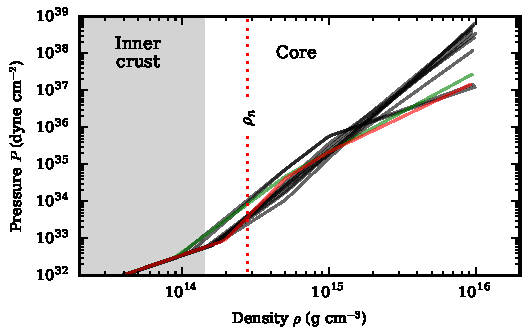
\includegraphics[width=7.5cm]{notes/eos/dense_eos.pdf}
\includegraphics[width=7.5cm]{notes/tov/mr.pdf}
\caption{\label{fig:core}
Core EoS.
}
\end{figure}

Outer core.
Density ranges $0.5 \nsat < \rho < 2\nsat$.
Several kilometers.
Neutrons with several per cent admixture of protons $p$ and electrons $e^{-}$.
Strongly degenerate.
Electrons form almost ideal Fermi gas.
Neutrons and protons, interacting via nuclear forces, constitute a strongly interacting Fermi liquid.

Inner core.
Where $\rho > 2\nsat$.
Appearance of muon.
Central density can be around $(10-15)\nsat$.
Very model dependent.
Main problem.

Here we consider few (relatively) modern descriptions for the dense matter equation of state.
%We follow the naming convention selected in Read et al.\cite{Read2010}, and divide the composition into: 
The EoSs can be divided into few different classes based on the particles that they consist of.
Here they are divided into matter consisting of
\begin{itemize}
    \item plain \npem nuclear matter, 
    \item normal nuclear matter spiced up with hyperons \hyperon,
    \item normal nuclear matter together with more exotic particles like pion and kaon condensates \pikaon,
    \item and matter consisting of (or normal matter spiced up with) quarks \quark.
\end{itemize}

For \npem we include models computed with
\begin{itemize}
    \item potential method using SLy effective nuclear interaction that is of Skyrme-type,\cite{SLy},
    \item four variational method EoSs, APR3/4\cite{APR} and WFF1/2\cite{WFF},
    \item two relativistic Brueckner-Hartree-Fock calculations, ENG\cite{ENG} and MPA1\cite{MPA},
    \item two relativistic mean-field theory, MS1 and MS1b (same as MS1 but with lower symmetry energy)\cite{MS}.
\end{itemize}

For hyperon models \hyperon we include
\begin{itemize}
    \item one variant of relativistic mean-field theory EoS H4\cite{H4}.
\end{itemize}

EoSs where mesons, like pion and kaon condensates \pikaon, are taken into account end up not being stiff enough.

Finally, for the hybrid nuclear matter and quark matter compositions \quark we include 
\begin{itemize}
    \item mixed APR nuclear matter and color-flavor-locked quark matter EoS ALF2.\cite{ALF}
\end{itemize}



\subsection{Why neutrons then?}
Let us first consider ideal gas of degenerate electron-proton-neutron plasma.
In a degenerate plasma all the quantum states are filled up all the way to the Fermi energy.
It is the Pauli exclusion principle that then prevents occupying all of these already taken quantum states.
Normal beta-decay mode for the neutrons, on the other hand, is $n \rightarrow p + e^{-} + \bar{\nu_{e}}$, that describes the possible path of how a neutron $n$ will decay into a proton $p$, electron $e^{-}$, and electron neutrino $\bar{\nu_{e}}$.
Such a decay is, however, blocked because there is no room for an emission of an extra electron $e^{-}$ or a proton $p$.\cite[see e.g.][]{Phillips94}

Let us then only focus on the decay of the most energetic neutrons with an energy equal to the Fermi energy $\ef(n)$.
Co-existence of neutrons, protons, and electrons is then guaranteed (at zero temperature) if 
\be
\ef(n) = \ef(p) + \ef(e^{-}).
\ee
Fermi momentum of a particle is related to its concentration via
\be
p_{\mathrm{F}} = \left( \frac{3n}{8\pi} \right)^{1/3} h,
\ee
where $n$ is the number density, and $h$ the Planck constant.
Massive neutrons and protons are to a good approximation non-relativistic up to a densities of $\nsat$, and hence energy is simply a sum of their rest mass energy and kinetic energy
\be
\ef(n) \approx m_n c^2 + \frac{p_{\mathrm{F}}(n)^2}{2 m_n },
\ee
and
\be
\ef(p) \approx m_p c^2 + \frac{p_{\mathrm{F}}(p)^2}{2 m_p }.
\ee
Electrons, on the other hand, are already ultra-relativistic, and so
\be
\ef(e^{-}) \approx p_{\mathrm{F}}(e^{-}) c^2.
\ee

\red{
Also note that $n_p = n_e$, as the star is electrically neutral.
From this we find relation of the $n_n/n_p \sim 1/200$ by taking into account the rest mass difference $m_p - m_n = 2.6 \mathrm{MeV}\,c^2$ at $\rho \sim \nsat$.
}
Thus, we conclude that the matter inside is neutron rich.


\subsection{Polytropes}
\red{Parameterize everything with polytropes.}

$P(\rho) = K \rho^{\gamma}$, $\gamma$ is a the polytropic index and is a measure of \emph{stiffness} of the EoS.
how strongly the matter responds to an increase in density with an increase in pressure





\section{Tolman-Volkoff-Oppenheimer equations}
Newtonian pressure gradient needed to oppose the gravity is
\be
\frac{dP}{dr} = -\frac{G m \rho}{r^2}.
\ee

\be
\frac{dm}{dr} = 4\pi r^2 \rho,
\ee

Taking into account the general relativistic corrections we get
\be
\frac{dP}{dr} = 
    -\frac{G M \rho}{r^2} \times 
    \frac{ (1 + P/\rho c^2)(1+4\pi r^3 P/m c^2) }
    {1-2 G m /r c^2 }.
\ee
Difference originates from the source of gravity:
in the Newtonian case it is the mass $m$, whereas in the General relativity it is the energy momentum tensor that depend both on the energy density and the pressure.
As a result, energy and pressure give rise to a gravitational fields.

Severness of the GR corrections can be estimated from the so called compactness parameter
\be
x = \frac{GM}{Rc^2} \approx 2.95~M/\Msun \km
\ee


It has an important consequence to the stability of neutron stars:
Successive increase in the pressure to counter the gravity is ultimately self-defeating.

\red{
Solution for a constant density $\rho_0$ gives
\be
P(r) = G \frac{2\pi}{3} \rho_0^2 (R^2 - r^2)
\ee
whereas the GR gives
\be
P(r) = \rho_0^2 c^2 \left[ \frac{ (1-u \left(\frac{r}{R} \right)^2 )^{1/2}
                        - (1-u)^{1/2} }{
                        3(1-u)^{1/2} - (1-u \left( \frac{r}{R} \right)^2 )^{1/2} } \right],
\ee
where $u = 2GM/Rc^2$.
}









